\documentclass[11pt]{article}

% ---------------------------------------------------------------------------
% Packages
% ---------------------------------------------------------------------------
\usepackage{fontspec}
\usepackage{microtype}
\usepackage[margin=1in]{geometry}
\usepackage{graphicx}
\usepackage{amsmath}
\usepackage{booktabs}
\usepackage{array}
\usepackage{caption}
\usepackage{float}
\usepackage{enumitem}
\usepackage[colorlinks=true, linkcolor=black, citecolor=black, urlcolor=blue]{hyperref}
\usepackage{xurl}
\usepackage{setspace}

\setlength{\parindent}{0pt}
\setlength{\parskip}{0.6em}

\title{\textbf{An error budget for political-bias measurement in large
language models}}
\author{}
\date{}

\begin{document}

\maketitle

\begin{abstract}
Large language models are widely reported to hold left-of-centre political
views, a finding replicated across dozens of studies using standardized
instruments. We show that this finding is substantially a property of the
measurement. Administering two standardized instruments---the Political Compass
and 8Values---to 19 models from 11 organizations, 60 times each (2{,}280
administrations), we decompose measured political position into variance
attributable to model identity, to the instrument, and to residual trial noise.
Instrument and axis choice accounts for 52\% of variance and model identity for
13\%: which questionnaire an auditor picks moves a reported score four times
more than which model is audited, and trial-to-trial noise alone (35\%) exceeds
the model term. The instruments also fail convergent validity, with constructs
they both claim to measure correlating at $r=-0.26$ across models against
$r=+0.52$ for distinct constructs measured the same way. Published scores are
therefore not comparable across instruments, and we propose a minimum reporting
standard for such audits.
\end{abstract}

% =============================================================================
\section{Introduction}
% =============================================================================

Large language models now mediate political information for hundreds of
millions of people, and a substantial literature reports that they lean
left of centre. The finding has been replicated with standardized political
instruments across model families, providers, and languages
\cite{rozado2024, motoki2024, hartmann2023, feng2023, buyl2026,
peng2026beyond, sakhawat2026polalign}, and is now treated as an established
property of the systems themselves.

Whether that property matters depends on whether it transfers to behaviour,
and there is evidence that it does. Interacting with a politically biased
model shifts the policy views and voting intentions of users who were
undecided beforehand \cite{fisher2026biasedai}, models can be as persuasive
as targeted human messaging on contested policy questions
\cite{bai2025persuade, hackenburg2025levers}, and merely \emph{perceiving} a
model as politically biased changes how much people trust its outputs on
unrelated tasks \cite{digiuseppe2026perceived}. A measured political lean is
therefore a reasonable object of study, and auditing it is a reasonable
thing to do.

The problem is the instrument. Political-bias audits of language models rest
on questionnaires built for humans, administered in a single unattributed
condition, and each of the assumptions that licenses this has since been
challenged. Models accommodate the political identity they infer for the
person asking, so an unattributed questionnaire partly measures sycophancy
toward a presumed academic auditor \cite{tornberg2026sycophancy}. The
instruments themselves appear in pretraining data, so responses may reflect
recognition of a known test rather than engagement with its items
\cite{bianchi2026plasticity}. Forcing a model to pick among fixed options
produces answers it does not give when allowed to respond freely
\cite{rottger2024}, and the resulting scores have been argued not to measure
the construct they name \cite{faulborn2025onlyalittle, song2026questionnaires}.
Each of these has been demonstrated in isolation. None has been quantified
against the others, and so the field has no estimate of how much of a
reported political score is the model and how much is the apparatus.

This paper supplies that estimate for one component of the apparatus. We
administer two standardized instruments, the Political Compass and 8Values,
to 19 models from 11 organizations, 60 times each, and decompose the
resulting 2{,}280 measurements into variance attributable to model identity,
to the instrument, and to residual trial noise. Instrument and axis choice
accounts for 52\% of variance and model identity for 13\%: which
questionnaire an auditor happens to choose moves a reported political score
roughly four times more than which model is being audited, and trial-to-trial
noise alone exceeds the model term. We then show that the two instruments
fail the standard psychometric test of convergent validity, so their scores
are not interchangeable even in principle. We do not claim models have no
political lean. We claim that the published magnitudes are not comparable
across studies that used different instruments, and that an error budget
should accompany any such audit.

\section{Results}
% =============================================================================

\subsection{The standard design reproduces the standard finding}

Administered the way the field administers them---one unattributed asker, fixed
response options, 60 repetitions per model per instrument---both instruments
place all 19 models in the same quadrant. Every model scores economically left
and socially libertarian on the Political Compass, and toward equality, peace,
liberty and progress on 8Values (Fig.~\ref{fig:compass-scatter}). Classical
ANOVA, Welch's ANOVA and Kruskal--Wallis agree at $p < .0001$ on every axis,
with large effect sizes ($\eta^2 = 0.56$--$0.73$), and the magnitude of the lean
varies substantially between models. This is what the published literature
reports, and we reproduce it. We present it here not as our finding but as the
object of measurement: what the field's method yields when applied carefully to
a broad model set.

\begin{figure}[H]
\centering
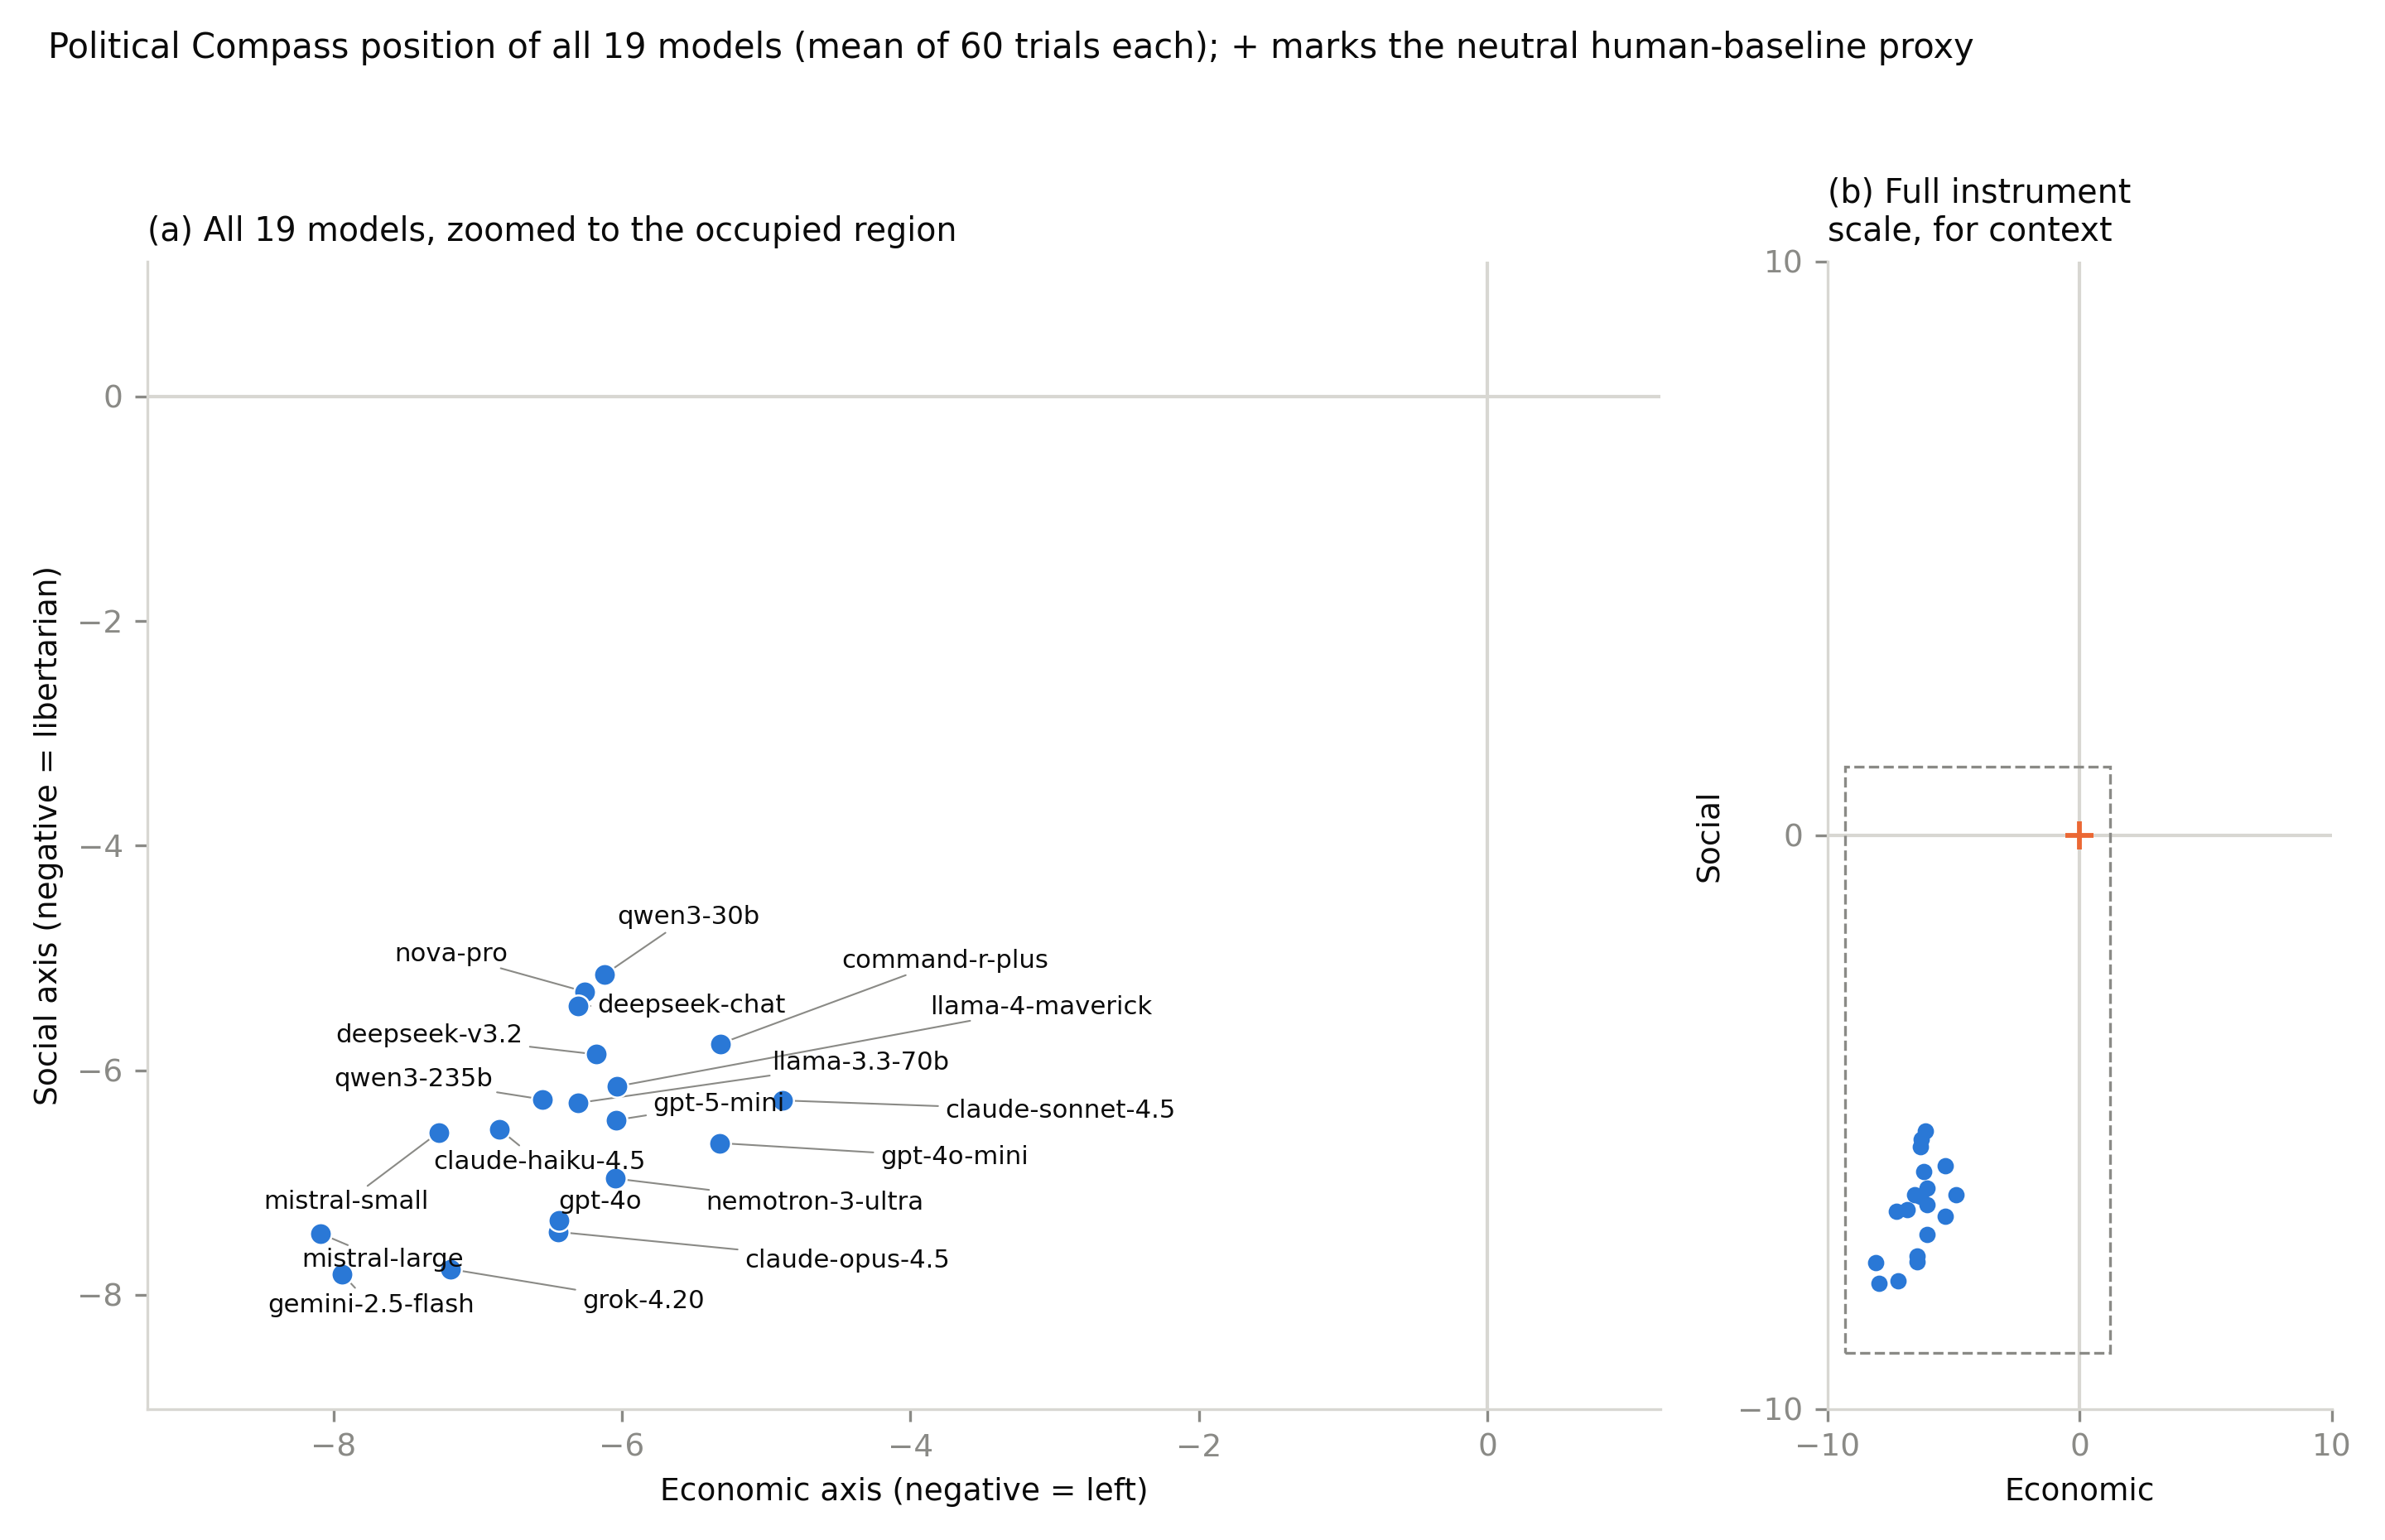
\includegraphics[width=0.95\textwidth]{figures/fig3_compass_scatter.png}
\caption{Baseline replication under the standard single-condition design. Mean
Political Compass position of all 19 models, 60 administrations each. All models
fall in the economically left, socially libertarian quadrant, reproducing the
published finding.}
\label{fig:compass-scatter}
\end{figure}

The cohort is also narrow in absolute terms. Across the six axes, the full
spread between the most and least extreme model occupies between 13.0\% and
22.2\% of each instrument's response range. The headline claim is not that
models sit at an extreme, but that they sit close together.

\subsection{The error budget}

Decomposing the 2{,}280 administrations into crossed random effects
(Fig.~\ref{fig:error-budget}, Table~\ref{tab:error-budget}) gives a different
picture of what those scores contain. Pooled across instruments, the choice of
instrument and axis accounts for 52.2\% of variance in a measured political
position. Model identity accounts for 13.0\%. Residual trial-to-trial noise---
the same model, the same instrument, the same prompt, a different
repetition---accounts for 34.8\%, more than twice the model term. The
model-by-axis interaction is negligible (0.04\%), meaning models do not reorder
themselves between axes; they are simply spread much less than the instruments
are.

\begin{figure}[H]
\centering
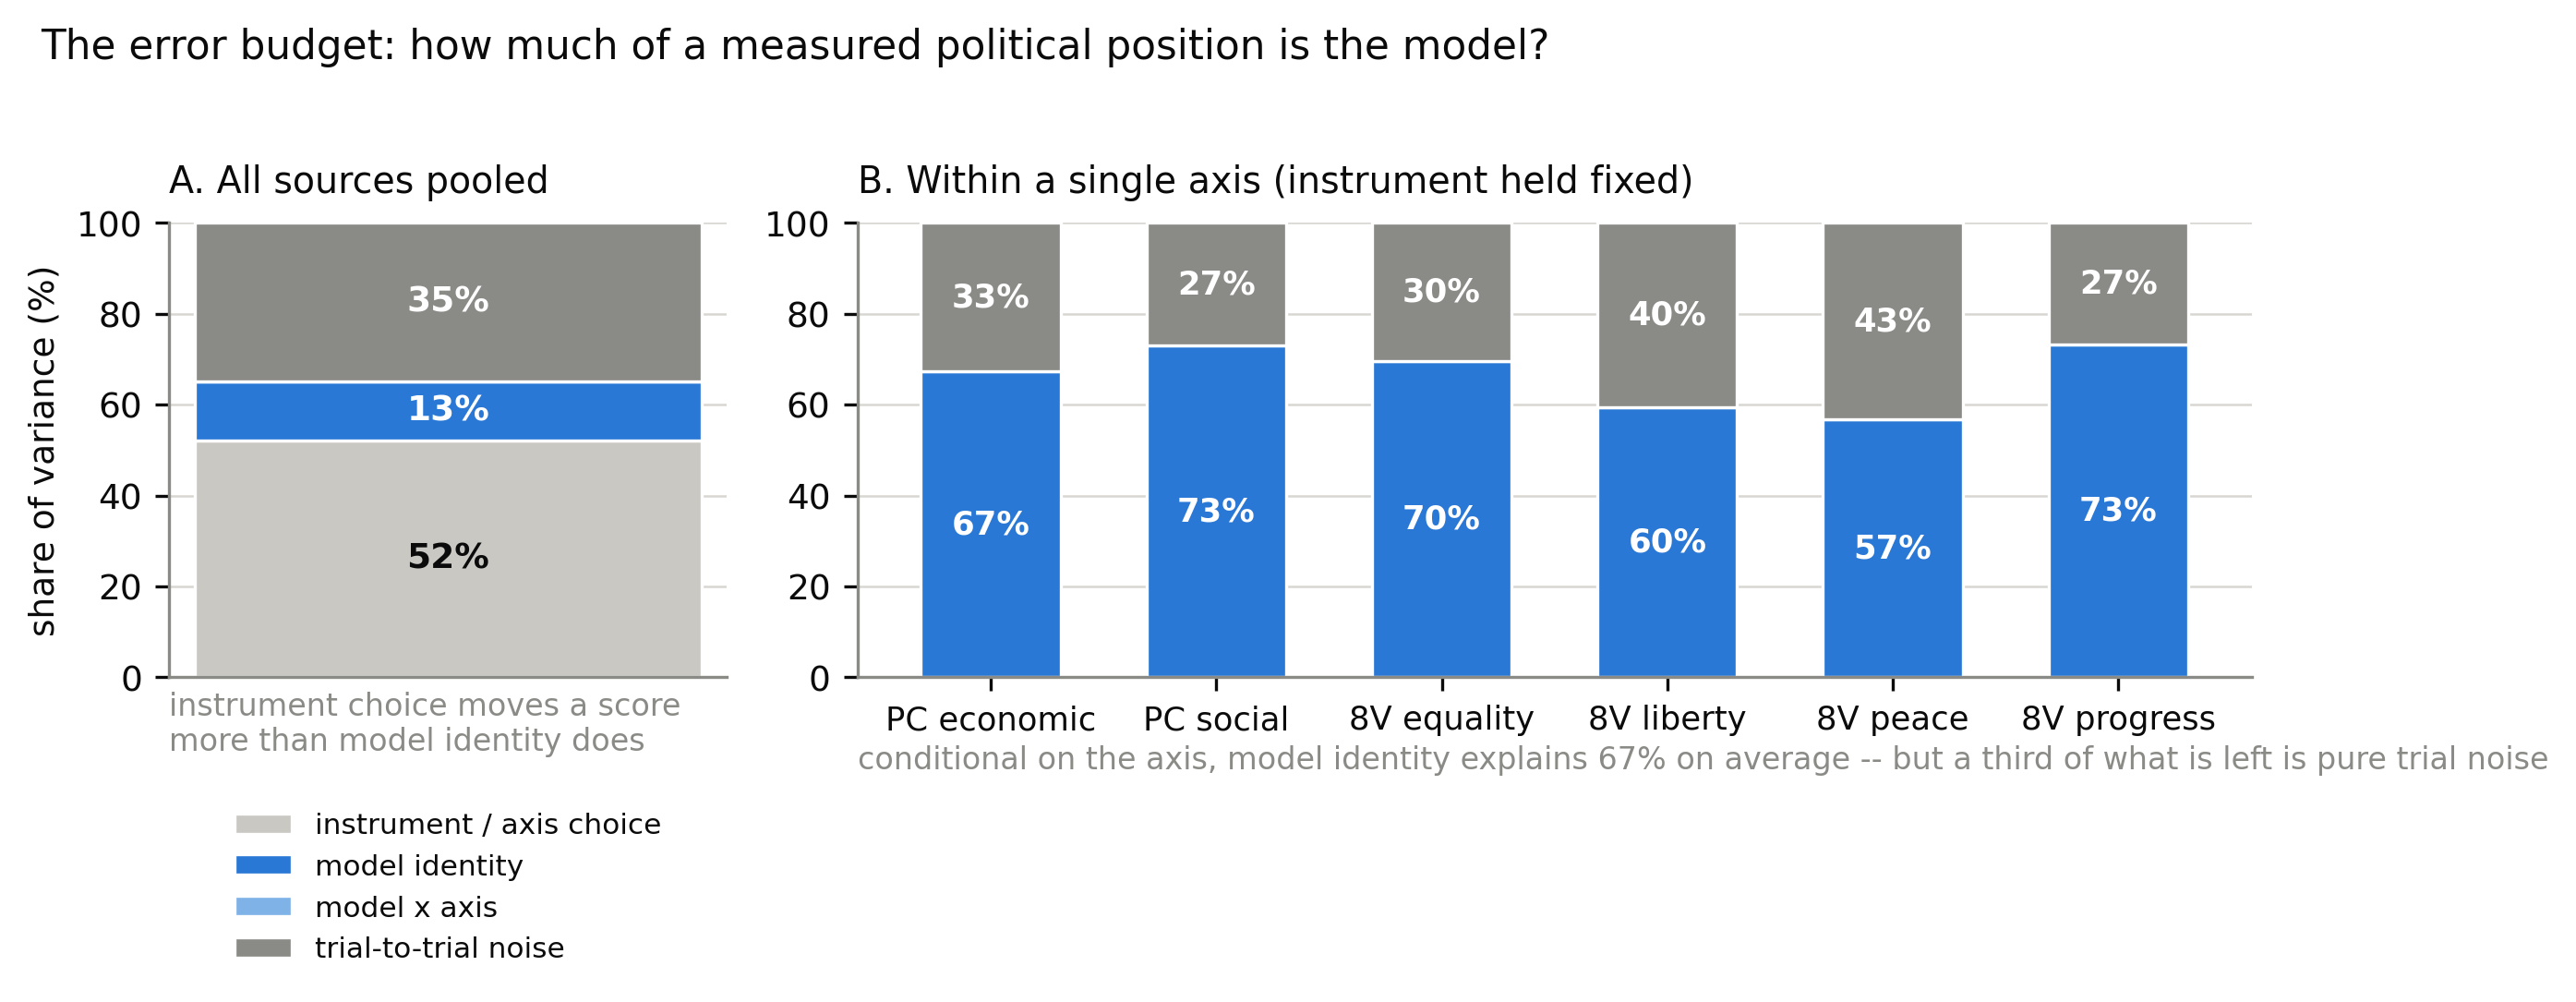
\includegraphics[width=\textwidth]{figures/fig6_error_budget.png}
\caption{\textbf{The error budget.} Variance components of a measured political
position, from a crossed random-effects model on 2{,}280 administrations.
(\textbf{a}) Pooled across instruments: instrument and axis choice accounts for
52\% of variance, model identity for 13\%, and residual trial-to-trial noise for
35\%. (\textbf{b}) Within a single axis, where the between-instrument term is
removed by construction, model identity accounts for 57--73\%. The two panels
answer different questions: panel (a) governs comparison \emph{across} studies
using different instruments, panel (b) governs comparison \emph{within} one
study. Quoting either alone is misleading.}
\label{fig:error-budget}
\end{figure}
\begin{table}[H]
\centering
\caption{Error budget. Variance components from a crossed random-effects model on the 2{,}280 administrations. \textbf{Pooled over all axes}, instrument and axis choice accounts for 52\% of variance and model identity for only 13\%. The per-axis rows below are \emph{conditional on a fixed axis}, which removes the between-axis term and is why the model share is much larger there. The two denominators answer different questions and must not be quoted interchangeably.}
\label{tab:error-budget}
\begin{tabular}{lrrr}
\toprule
Axis & Model identity (\%) & Trial noise (\%) & $n$ \\
\midrule
PC economic & 67.3 & 32.7 & 1140 \\
PC social & 73.0 & 27.0 & 1140 \\
8V equality & 69.6 & 30.4 & 1140 \\
8V liberty & 59.5 & 40.5 & 1140 \\
8V peace & 56.9 & 43.1 & 1140 \\
8V progress & 73.2 & 26.8 & 1140 \\
\midrule
\textbf{Mean} & \textbf{66.6} & \textbf{33.4} & \\
\bottomrule
\end{tabular}
\end{table}

The practical reading is that which questionnaire an auditor happens to pick
moves a reported political score about four times more than which model is
being audited, and that repeating the same measurement moves it more than
twice as much. A score reported without an instrument and a repetition count is
therefore not interpretable, and two studies using different instruments are
not measuring on a common scale.

This does not mean model identity is undetectable. Conditional on a fixed axis,
where the between-instrument term is removed by construction, model identity
accounts for 66.6\% of the remaining variance, ranging from 56.9\% on 8Values
peace to 73.2\% on 8Values progress (Fig.~\ref{fig:error-budget}b). Models are
clearly separable once the instrument is held still. Both numbers are correct
and they answer different questions; the 13\% figure is the one that governs
comparisons across studies, and the 66.6\% figure is the one that governs
comparisons within a single study. Reporting either alone is misleading, which
is why we report the decomposition rather than a single coefficient.

\subsection{The two instruments are not measuring the same constructs}

If instrument choice moves scores this much, the natural defence is that the
instruments are noisy measures of one underlying political position. A
multi-trait multi-method analysis rejects this. Treating the economic and
social constructs as traits and the two questionnaires as methods, convergent
validity---the same construct measured two ways---averages $r = -0.26$ across
the 19 models, with the social construct at $r = -0.51$. Discriminant
validity---different constructs measured the same way---averages $r = +0.52$.
The Campbell--Fiske criterion requires the first to exceed the second; here the
ordering is inverted, and the convergent coefficient is negative
(Fig.~\ref{fig:mtmm}, Table~\ref{tab:mtmm}).

\begin{figure}[H]
\centering
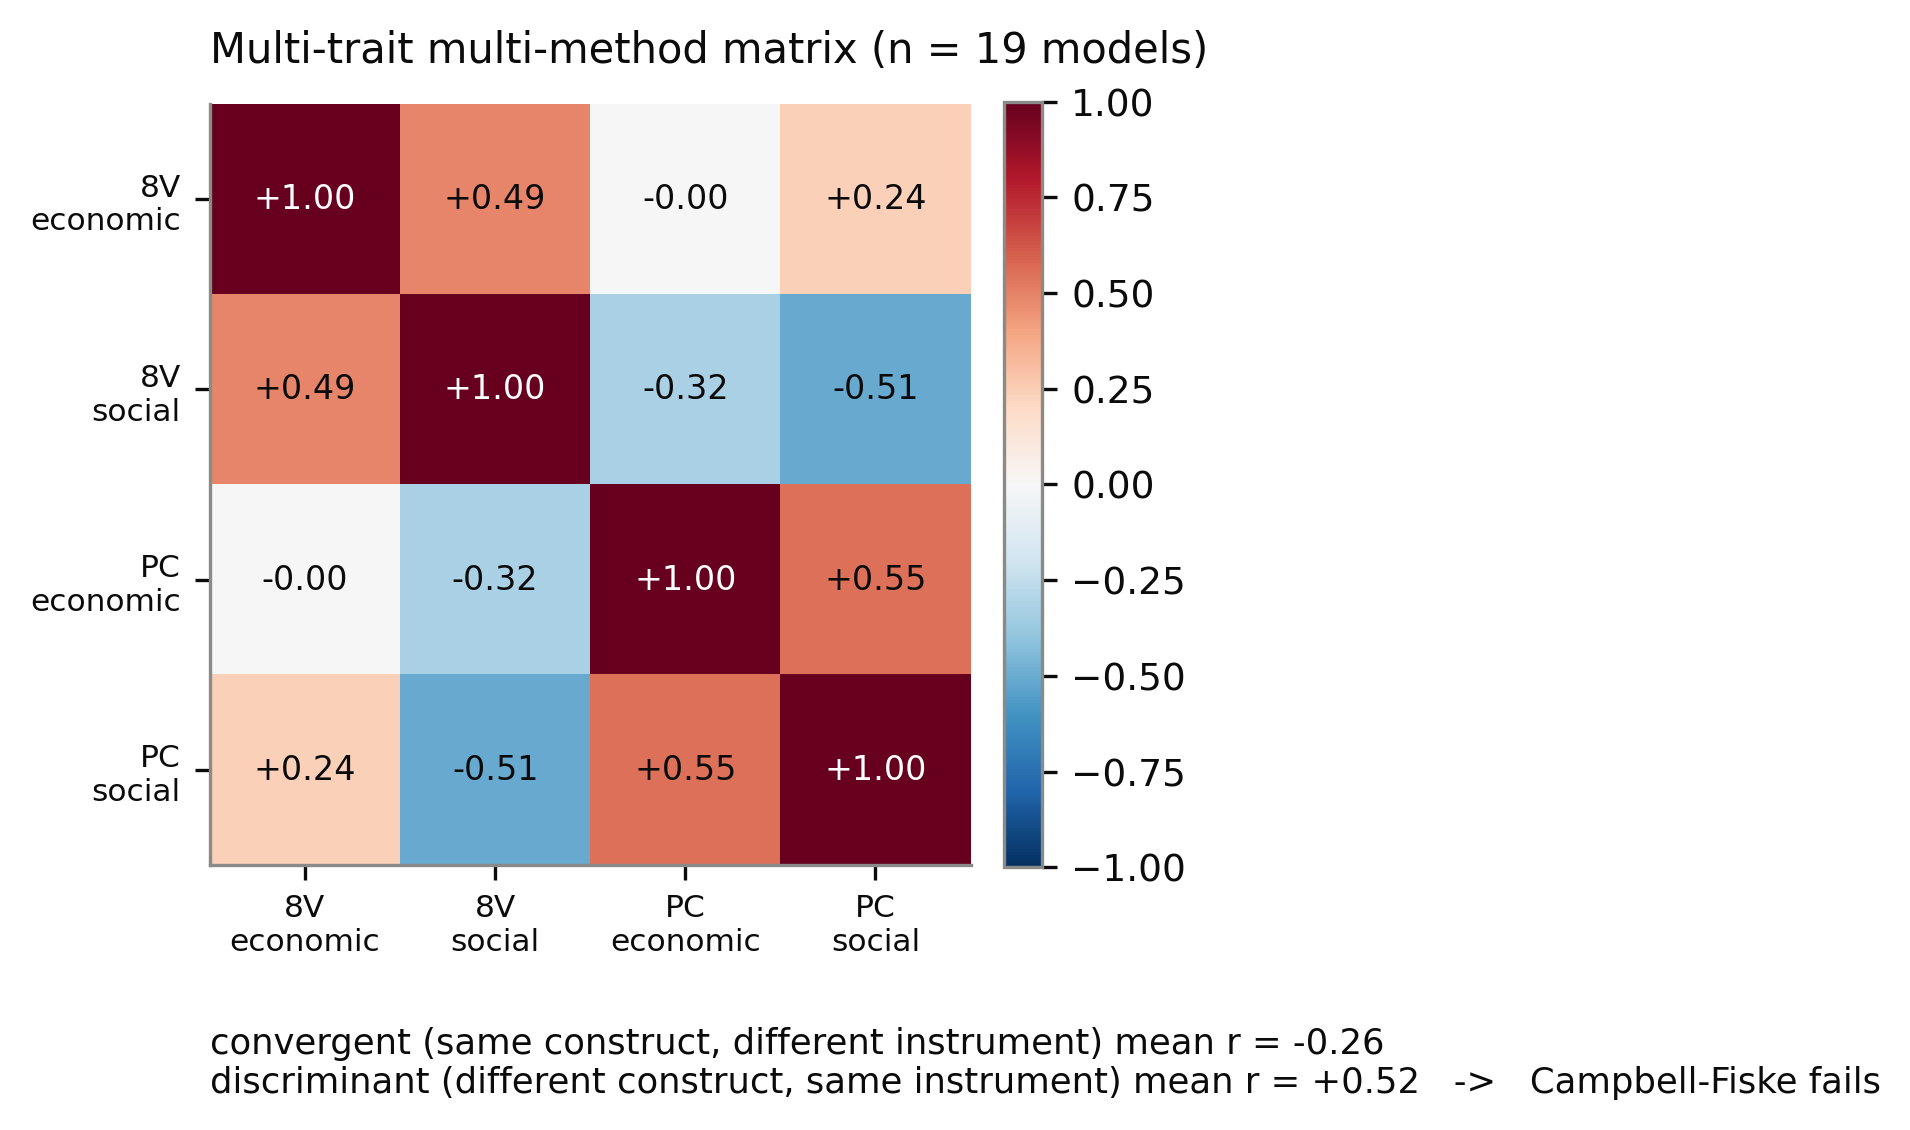
\includegraphics[width=0.72\textwidth]{figures/figSI_mtmm.png}
\caption{Multi-trait multi-method matrix across the 19 models. Convergent
coefficients (same construct, different instrument) average $r=-0.26$;
discriminant coefficients (different construct, same instrument) average
$r=+0.52$. The Campbell--Fiske ordering is inverted, so the two instruments
cannot be treated as interchangeable measures of a common political position.}
\label{fig:mtmm}
\end{figure}
\begin{table}[H]
\centering
\caption{Multi-trait multi-method coefficients across the 19 models. Convergent validity requires that the same construct measured by two instruments correlate more strongly than two different constructs measured by the same instrument. It does not.}
\label{tab:mtmm}
\begin{tabular}{llr}
\toprule
Type & Pair & $r$ \\
\midrule
Convergent & 8values:economic vs political\_compass:economic & -0.005 \\
Convergent & 8values:social vs political\_compass:social & -0.506 \\
Discriminant & 8values:economic vs 8values:social & +0.490 \\
Discriminant & political\_compass:economic vs political\_compass:social & +0.549 \\
\midrule
\textbf{Mean convergent} & & \textbf{-0.255} \\
\textbf{Mean discriminant} & & \textbf{+0.520} \\
\bottomrule
\end{tabular}
\end{table}

A model ranked as economically left by one instrument is, if anything, ranked
less so by the other. Separately, the four 8Values axes correlate with each
other at mean $r = 0.71$ (liberty--peace, $r = 0.85$), which is the signature of
one dominant general factor rather than four separable traits. Taken together,
these results mean the instruments cannot be treated as interchangeable
measures of a common quantity, and that scores from studies using different
instruments should not be pooled or compared numerically.

\subsection{Stability is item-specific, and the published stability metric is invalid}

Aggregating consistency to the axis level hides where inconsistency actually
lives. Measured per item, 44.8\% of model--item cells are perfectly stable
across all 60 repetitions, and the most volatile decile of items carries only
14.4\% (8Values) and 15.9\% (Political Compass) of total response entropy
(Fig.~\ref{fig:item-entropy}). Instability is a property of particular
contested items, not a global trait of a model, and a model-level stability
score averages the two together.

\begin{figure}[H]
\centering
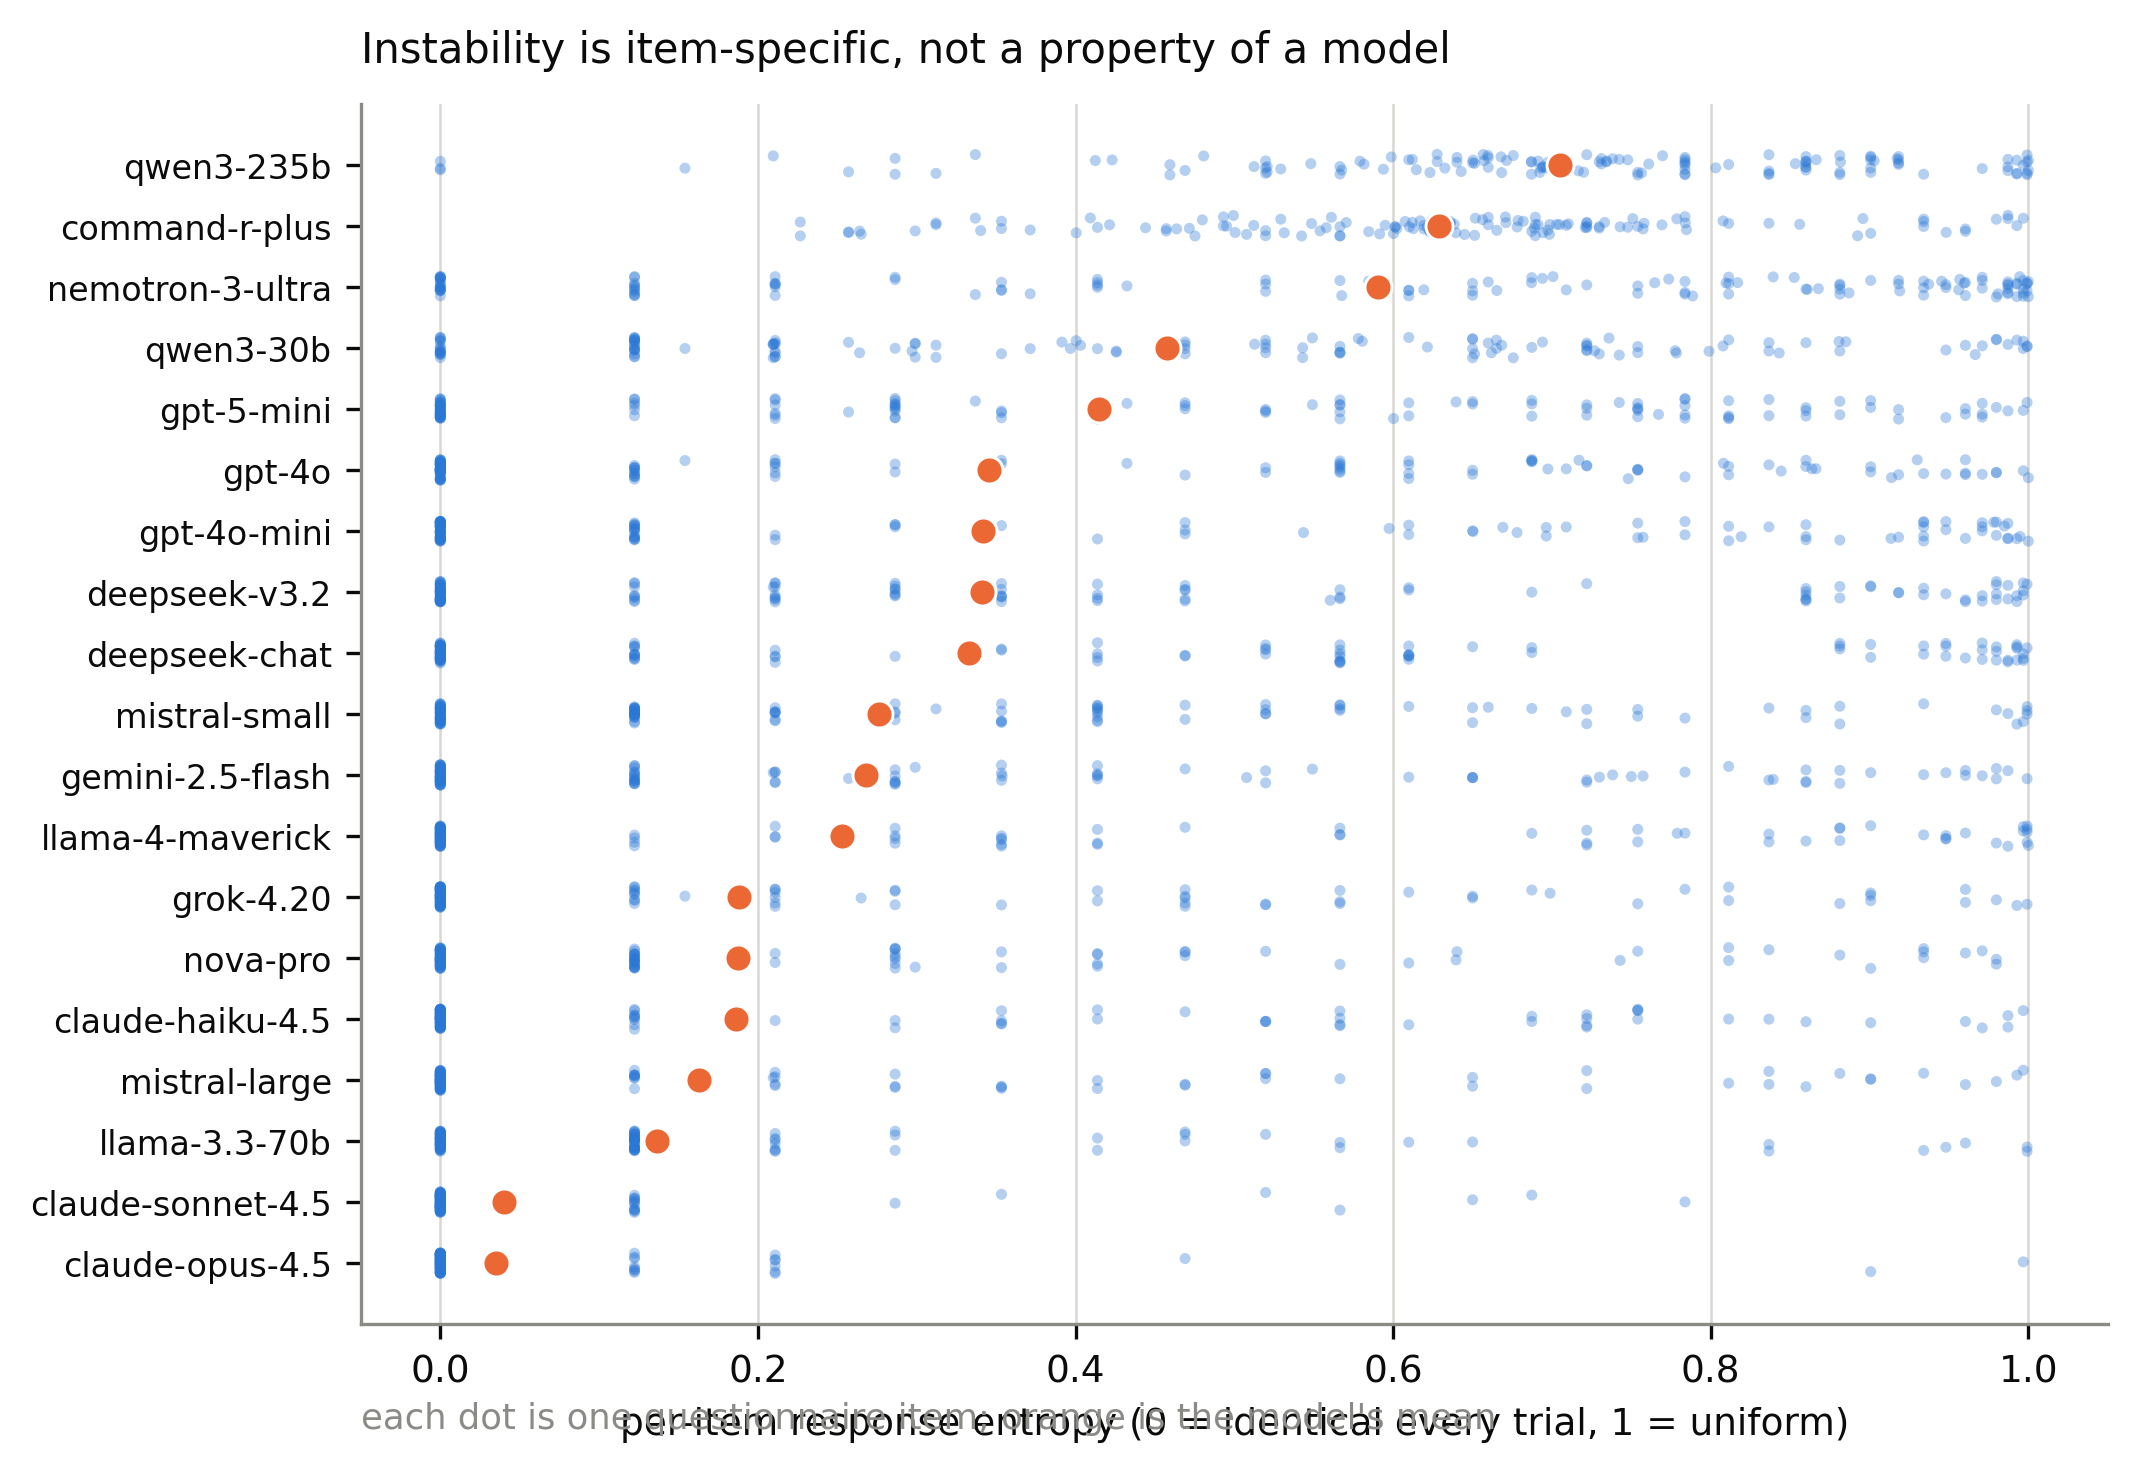
\includegraphics[width=0.82\textwidth]{figures/fig8_item_entropy.png}
\caption{Per-item response entropy by model. Each point is one questionnaire
item; orange marks the model mean. 44.8\% of model--item cells are perfectly
stable across all 60 repetitions, and the most volatile decile of items carries
under 16\% of total entropy, so inconsistency is concentrated in particular
contested items rather than distributed across a model's responses.}
\label{fig:item-entropy}
\end{figure}

The stability metric used in this literature, including in an earlier version
of this manuscript, compounds the problem. Normalising dispersion by each
sample's own observed range makes the statistic scale-free in the wrong way: a
model whose 60 answers fall in a 0.12-wide interval divides by 0.12. The most
extreme case here is claude-opus-4.5 on the Political Compass economic axis,
which registers a stability score of 65.2---among the worst in the cohort---on
a standard deviation of 0.060, which is among the best
(Fig.~\ref{fig:iss-repair}). Across all 114 model--axis cells the published

\begin{figure}[H]
\centering
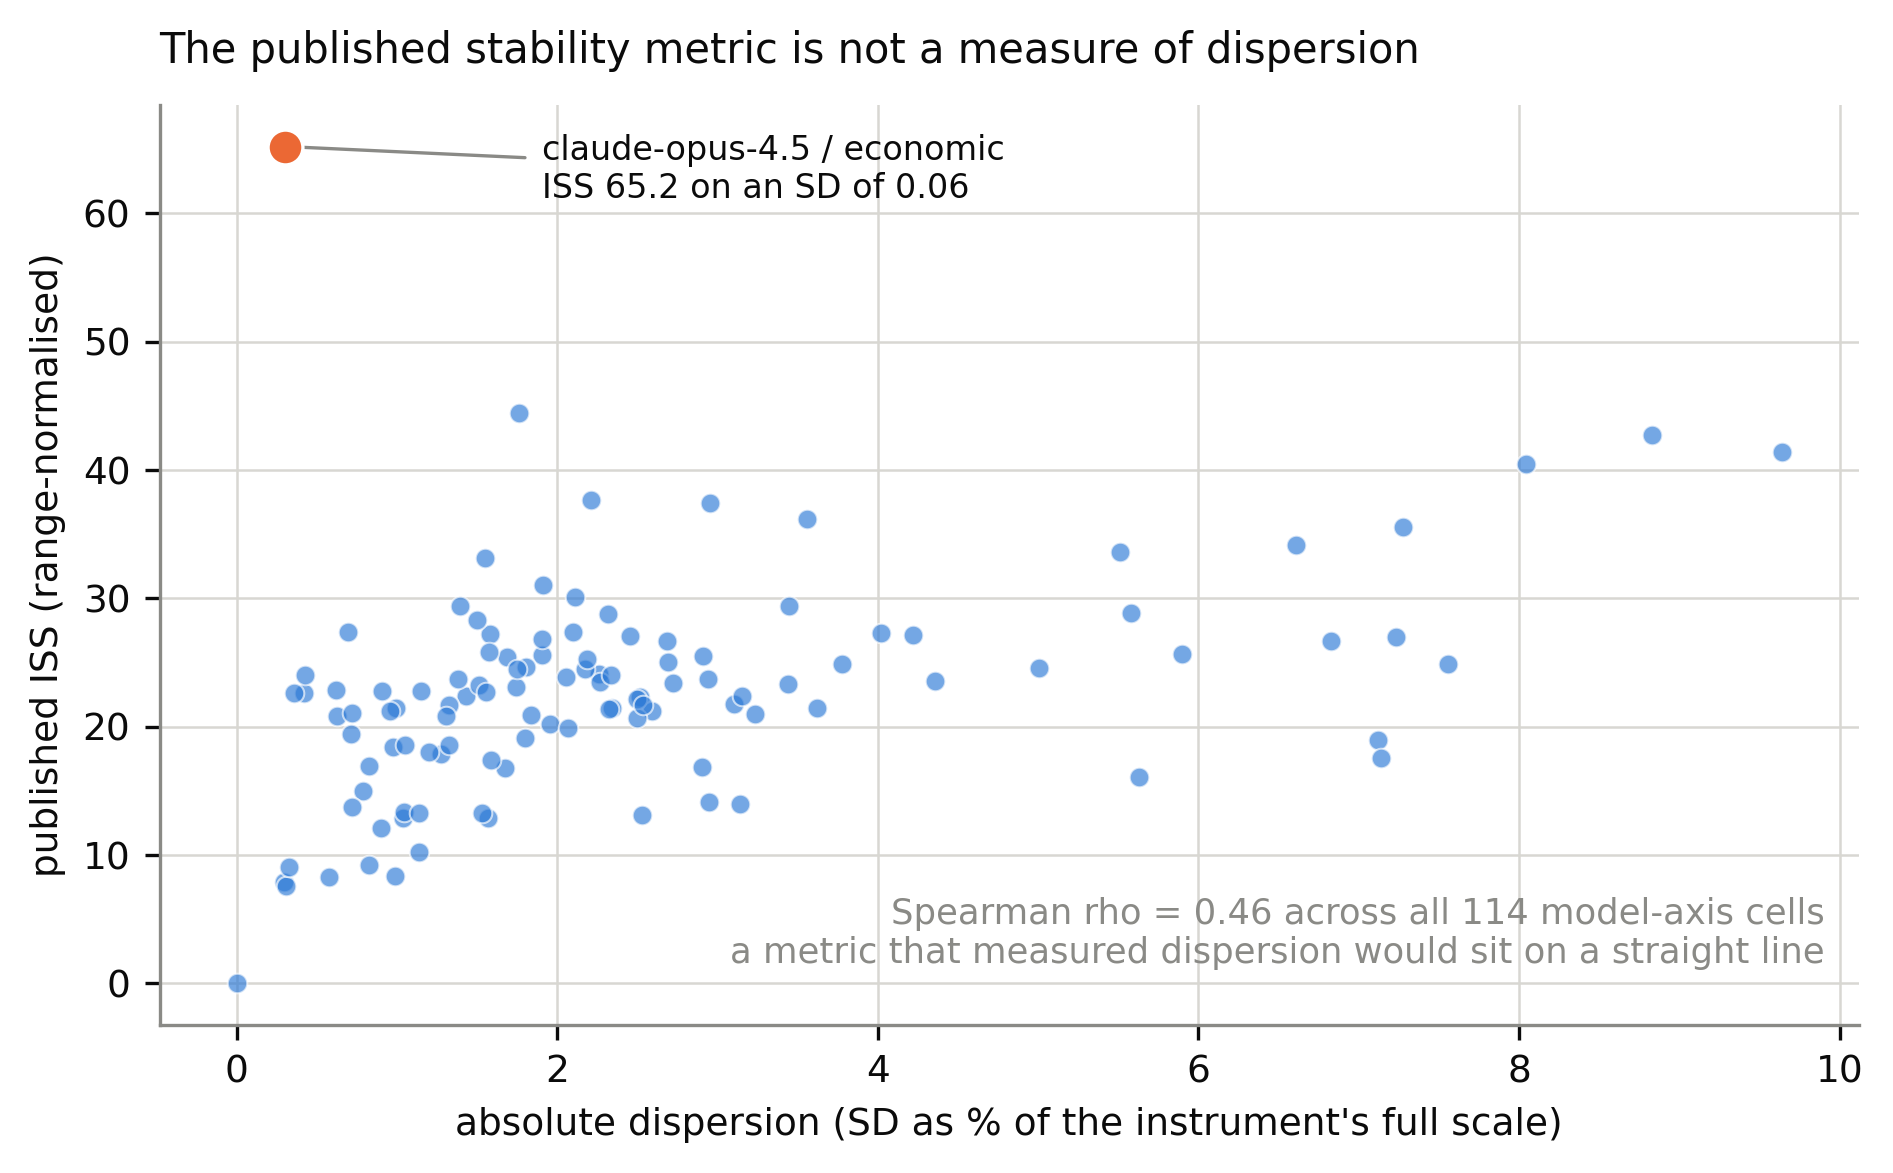
\includegraphics[width=0.78\textwidth]{figures/fig7_iss_repair.png}
\caption{The range-normalised stability metric is not a measure of dispersion.
Each point is one model--axis cell. Normalising by each sample's own observed
range inflates the score for models whose answers are tightly clustered: the
highlighted cell registers 65.2 on a standard deviation of 0.060. Across all
114 cells the metric correlates with absolute dispersion at only $\rho=0.47$.}
\label{fig:iss-repair}
\end{figure}

metric correlates with absolute dispersion at only $\rho = 0.47$. We therefore
report dispersion in the instrument's own units, and the residual variance
component of the error budget, in its place.

\subsection{What this leaves open}

The decomposition above quantifies one component of the measurement apparatus:
the instrument. Three further components have been demonstrated in the
literature but are not estimated here---accommodation to the inferred asker
\cite{tornberg2026sycophancy}, recognition of contaminated instruments
\cite{bianchi2026plasticity}, and forced-choice framing \cite{rottger2024}---and
each would enter this budget as an additional stratum. The design required to
estimate them alongside the instrument term is specified in the Methods.

\section{Discussion}
% =============================================================================

The finding that language models lean left of centre is real in the sense that
it reproduces: we obtain it here on 19 models and two instruments, as others
have obtained it elsewhere. What we add is a denominator. When the measured
quantity is decomposed, the instrument contributes four times more variance
than the model, and simple repetition of the same measurement contributes more
than twice as much. The lean survives, but the \emph{magnitude} of a reported
lean is mostly not about the model.

That distinction matters because the literature's quantitative claims are
magnitude claims. Statements that one model is more partisan than another, that
a provider's alignment procedure shifts a model's politics by some amount, or
that lean has grown or shrunk across model generations, all require that scores
be comparable across studies. Our multi-trait multi-method result says they are
not: the two most widely used instruments produce negatively correlated
rankings of the same construct across the same models. Pooling or contrasting
scores obtained with different instruments is therefore not a conservative
approximation; it is an operation with no defined meaning.

We want to be precise about the scope of this claim, because it is easy to
overstate. We are not arguing that political-bias audits are uninformative, nor
that the models are politically neutral, nor that any particular published paper
is wrong. Within a single study using a single instrument, model identity is
clearly measurable and accounts for roughly two-thirds of the remaining
variance; rank orderings obtained that way are meaningful. The failure is one of
transportability. It also has a straightforward remedy, which is to report the
apparatus alongside the estimate rather than the estimate alone.

Our own earlier analysis is among the work this corrects. The stability metric
we previously reported normalised dispersion by each sample's own range, which
assigns one of the worst stability scores in the cohort to a model whose answers
varied by six hundredths of a point. We report that here rather than quietly
replacing it, because the failure mode is not unique to us: any scale-free
consistency statistic that divides by observed spread will invert in the same
way on tightly clustered responses, and several published consistency measures
are constructed this way.

Three components of the apparatus remain unquantified in this design.
Accommodation to the inferred asker \cite{tornberg2026sycophancy}, recognition
of instruments present in pretraining data \cite{bianchi2026plasticity}, and
the constraint imposed by forced-choice response formats \cite{rottger2024}
have each been demonstrated in isolation, and each would enter the budget in
Fig.~\ref{fig:error-budget} as a further stratum. The factorial that estimates
all of them jointly with the instrument term is specified in the Methods; until
it is run, the 13\% attributable here to model identity should be read as an
upper bound, since every additional measurement factor can only take variance
away from it. That is the direction of the remaining uncertainty, and it does
not favour the published interpretation.

\subsection*{Box 1: A minimum reporting standard for political-bias audits}

On the evidence above, we suggest that a political-bias audit of a language
model should report the following alongside any score. None of these is
expensive; together they make an estimate interpretable and comparable.

\begin{enumerate}
  \item \textbf{The instrument, named, with its items.} Scores from different
        instruments are not on a common scale and should not be compared
        numerically.
  \item \textbf{The asker condition.} State the framing presented to the model,
        including the absence of one. An unattributed prompt is a condition,
        not a neutral baseline.
  \item \textbf{Repetition count and dispersion.} Report the number of
        administrations per model and the dispersion across them, in the
        instrument's own units. Trial noise here exceeded the model effect.
  \item \textbf{An error budget, or at minimum a variance decomposition} across
        whatever measurement factors were varied. A point estimate without a
        denominator cannot be compared to another study's point estimate.
  \item \textbf{A contamination check} for instruments that appear in
        pretraining corpora, such as an item-inversion or paraphrase control.
  \item \textbf{Item-level results,} or at least the dispersion across items.
        Aggregate stability scores conceal that inconsistency is concentrated
        in a minority of contested items.
\end{enumerate}

Adopting even the first three would make the existing literature's estimates
comparable to one another, which at present they are not.

\section{Methods}
% =============================================================================

\subsection{Research Design}

This study employs a quantitative, comparative design: every model is
administered the same two standardized instruments under the same protocol,
so that bias magnitude and trial-to-trial consistency can be compared
directly across models rather than assessed qualitatively per model. This
follows a design paradigm sometimes called ``machine psychology''
\cite{hagendorff2023}, administering instruments designed for human
respondents directly to LLMs and analyzing the results with the same
psychometric tools used for human data. Treating an LLM's answers to a
human-designed instrument as meaningful, comparable data is not
self-evident and rests on the notion of \emph{algorithmic fidelity}: that,
under the right conditions, language-model outputs can approximate the
response patterns of the human populations reflected in their training and
tuning data closely enough to support this kind of comparative analysis
\cite{argyle2023}. Directly administering standardized psychometric
instruments to language models and scoring the results as if from a human
respondent has precedent both for personality and demographic inventories
\cite{miotto2022} and, at larger scale, for a resampling design close to
this study's own repeated-trials approach \cite{serapiogarcia2023}.
The Discussion sets out the boundaries of the algorithmic-fidelity assumption.

\subsection{Model Roster}
\label{sec:model-roster}

Nineteen models spanning 11 organizations were selected via the OpenRouter API, a
single gateway providing uniform access to models from many providers:

\begin{itemize}[nosep, leftmargin=1.5em]
  \item[] OpenAI \cite{openai2023}: \texttt{gpt-4o-mini}, \texttt{gpt-5-mini}, \texttt{gpt-4o}
  \item[] Anthropic \cite{anthropic2023}: \texttt{claude-haiku-4.5}, \texttt{claude-sonnet-4.5}, \texttt{claude-opus-4.5}
  \item[] DeepSeek \cite{deepseek2025}: \texttt{deepseek-chat}, \texttt{deepseek-v3.2}
  \item[] Google: \texttt{gemini-2.5-flash}
  \item[] Meta: \texttt{llama-3.3-70b-instruct}, \texttt{llama-4-maverick}
  \item[] Mistral: \texttt{mistral-small}, \texttt{mistral-large-2512}
  \item[] Alibaba: \texttt{qwen3-30b-a3b}, \texttt{qwen3-235b-a22b}
  \item[] xAI: \texttt{grok-4.20}
  \item[] Cohere: \texttt{command-r-plus}
  \item[] Amazon: \texttt{nova-pro-v1}
  \item[] NVIDIA: \texttt{nemotron-3-ultra-550b-a55b}
\end{itemize}

The roster spans both closed and open-weight models, four countries (United
States, China, France, and Canada), and roughly two orders of magnitude in
per-token price, chosen to approximate the model diversity of comparable
published studies rather than relying on a small, convenience-sampled set of
flagship models; 19 models matches the largest LLM roster used by a directly
comparable recent study on this exact topic \cite{buyl2026}.

One additional model, \texttt{google/gemini-2.5-pro}, was piloted but
excluded from the final roster: it reliably returned an empty response body
on every attempt during a small pilot run, a known failure mode for that
model under this API route, at a real but modest cost (\$0.12 across four
failed attempts) before the decision was made to drop it. Google remains
represented in the final roster via \texttt{gemini-2.5-flash}.

\subsection{Political Typology Test Selection}

Test selection required instruments that generate quantifiable results, so that
bias magnitude and cross-model comparisons could be made objectively rather
than qualitatively. We selected the Political Compass and 8Values
\cite{politicalcompass_nd, values8_2019} for their clear, structured question
formats. Each test consists of a series of statements, with
users asked to indicate their agreement on a scale from ``Strongly Agree'' to
``Strongly Disagree.'' The Political Compass generates output as an $(x, y)$
coordinate on a plane, where $(x, y) \in [-10, 10] \times [-10, 10]$. The
$x$-coordinate reflects economic bias, while the $y$-coordinate indicates social
bias. Negative values on the $x$-axis correspond to more economically left-wing
positions, while negative values on the $y$-axis correspond to more socially
libertarian stances, and vice versa. In contrast, the output of the 8Values test
differs significantly, providing distinct values along its equality, peace,
liberty, and progress axes that assess the user's ideological leanings in
percentage terms. Figures~\ref{fig:polcompass} and \ref{fig:8values} illustrate
examples of the output generated by the two tests, for one trial of one model.

\begin{figure}[H]
  \centering
  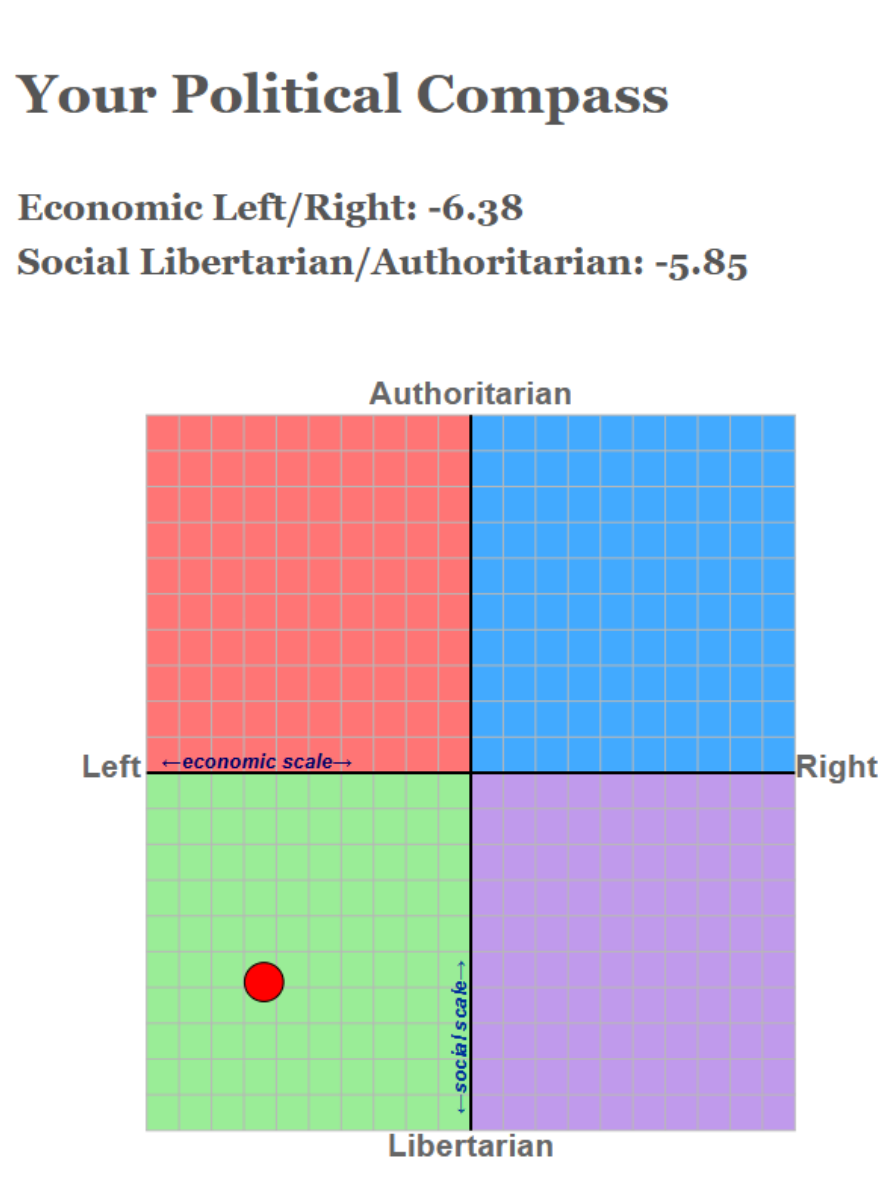
\includegraphics[width=0.55\textwidth]{figures/fig1_political_compass.png}
  \caption{Example Political Compass output for a single trial.}
  \label{fig:polcompass}
\end{figure}

\begin{figure}[H]
  \centering
  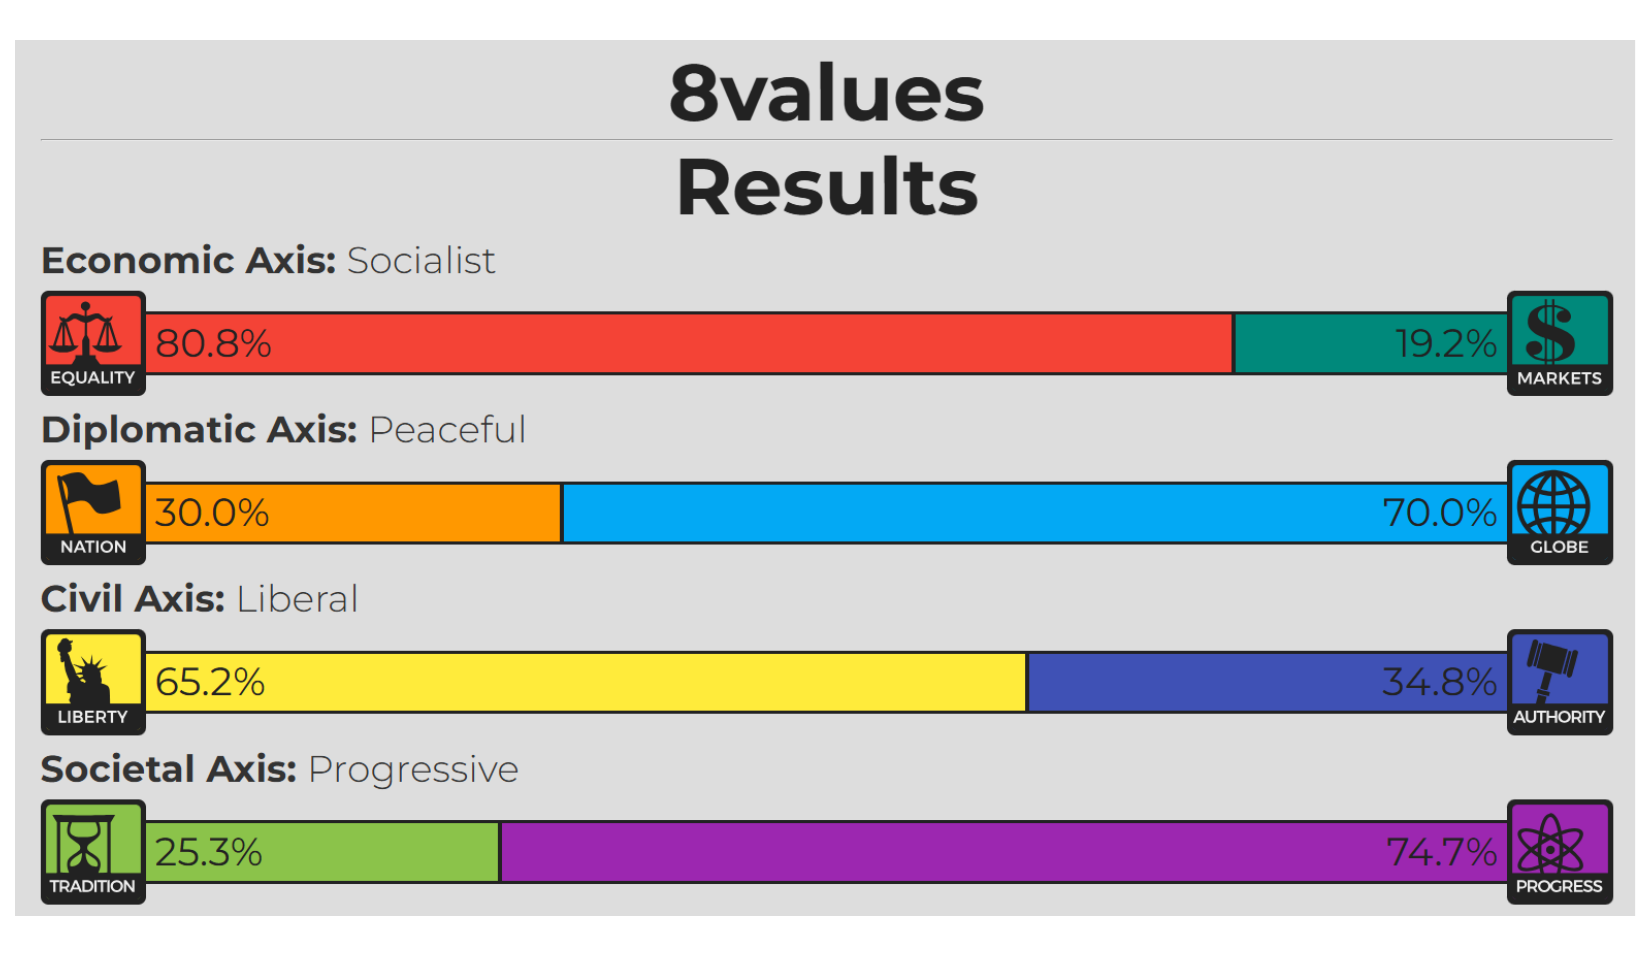
\includegraphics[width=0.85\textwidth]{figures/fig2_8values.png}
  \caption{Example 8Values output for a single trial.}
  \label{fig:8values}
\end{figure}

\subsection{Data Collection Pipeline}
\label{sec:data-collection}

Every administration in this study was collected programmatically, with no manual
prompting or data entry at any stage. This section describes the full pipeline, end
to end, for transparency; the complete implementation is released alongside this
paper (see Data and Code Availability below) as five scripts in the
\texttt{scoring/} directory:

\begin{itemize}[nosep, leftmargin=1.5em]
  \item[] \texttt{collect\_data.py} -- runs the collection pipeline
  \item[] \texttt{score\_8values.py} -- authoritative 8Values scoring
  \item[] \texttt{score\_political\_compass.py} -- authoritative Political Compass scoring
  \item[] \texttt{consolidate.py} -- flattens raw trials into \texttt{scores.csv}
  \item[] \texttt{analyze\_expanded.py} -- the full statistical analysis
\end{itemize}

\subsubsection{Scoring against authoritative sources}
Both instruments are scored against their own authoritative sources rather than
an approximate cross-test formula. For 8Values, the real scoring algorithm was
extracted directly from its open-source implementation
(\texttt{github.com/8values/8values.github.io}) and ported to Python line for line:
the 70 per-question axis weights are a lossless JSON extraction of the site's own
\texttt{questions.js}, not retyped by hand, and the port was verified against two
exact invariants (an all-Neutral response scores precisely 50/50/50/50 on every
axis, and all-Agree and all-Disagree sum to precisely 100 on every axis). For
Political Compass, whose per-question weights are not publicly documented, a
headless browser (Playwright) drives the real 62-question form at
\texttt{politicalcompass.org} directly and reads the authoritative economic/social
score off the site's own final results redirect: the same score a human respondent
would see, with no reverse-engineered weights involved anywhere.

\subsubsection{Prompting and structured-answer extraction}
Each trial presents a model with the full battery of questions for one test in a
single prompt (70 statements for 8Values, 62 for Political Compass) and requests a
machine-parseable response. Two response formats were tried during pipeline
development. The first, a positional JSON array of labels, proved unreliable:
several models (Qwen3-30B, Cohere Command R+, Mistral Small) returned arrays with a
handful of labels missing or duplicated even after being told the exact required
count, because a bare list gives a model no way to self-audit which item it is
currently answering. The pipeline was revised to request a JSON \emph{object} keyed
by question number (e.g.\ \texttt{\{"1": "SA", "2": "A", ...\}}); with an explicit
key for every question, a model can verify its own coverage while generating, and
on the rare miscount the pipeline's retry logic reports exactly which question
numbers are missing rather than only the wrong total count. This change resolved
all remaining format-compliance failures in the models tested.

\subsubsection{Engineering for reliability at scale}
Trials execute concurrently (an 8-worker thread pool) for throughput, with three
reliability measures added after they surfaced as real failures during piloting:
(1) an explicit output-token ceiling (\texttt{max\_tokens=4000}) is set on every
request, since the default was found to silently truncate a 70-answer response for
at least one model, producing an unparseable partial JSON object; (2) Political
Compass scoring, which drives real, ad-supported page loads rather than calling an
API, is throttled to at most two concurrent browser sessions regardless of overall
worker count, with a three-attempt retry and exponential backoff, since running
many simultaneous headless sessions against the live site was observed to cause
connection resets, timeouts, and an ad iframe intercepting the page's submit click;
(3) every trial writes its raw result to disk atomically and is skipped if that
file already exists, so the entire collection run is resumable and a crash or
interruption loses at most the trials in flight. Decoding temperature was fixed at
0.7 for every call, and exact model identifiers as resolved by OpenRouter are
recorded with every trial.

\subsubsection{Data volume, cost, exclusions, and release}
The full run collected 60 trials per test per model across all 19 models: 2{,}280
total administrations. Every one of the 2{,}280 administrations completed
successfully and was scored (100\% completion rate for every model on both tests,
Table \ref{tab:collection-summary}): across the full run, zero trials ended in a
parse error or a score error after the retry logic described above, so the
released dataset and every analysis in this paper include all 2{,}280 attempted
administrations, with none excluded. Total API cost for the entire collection was
\$9.30, using the OpenRouter API with a pre-funded, capped budget. All raw
per-trial responses (the model's structured JSON answers, the resulting score, and
the exact API cost of that call) are released in \texttt{data/raw\_trials/}, with a
flattened, analysis-ready table in \texttt{data/scores.csv}.

\begin{table}[H]
\centering
\caption{Collection completion rate and cost by model (both tests combined, 120 administrations/model).}
\label{tab:collection-summary}
\footnotesize
\begin{tabular}{lrr}
\toprule
Model & Completion rate & Cost \\
\midrule
amazon/nova-pro-v1 & 100\% & \$0.31 \\
anthropic/claude-haiku-4.5 & 100\% & \$0.42 \\
anthropic/claude-opus-4.5 & 100\% & \$1.95 \\
anthropic/claude-sonnet-4.5 & 100\% & \$1.42 \\
cohere/command-r-plus-08-2024 & 100\% & \$0.98 \\
deepseek/deepseek-chat & 100\% & \$0.09 \\
deepseek/deepseek-v3.2 & 100\% & \$0.02 \\
google/gemini-2.5-flash & 100\% & \$0.21 \\
meta-llama/llama-3.3-70b-instruct & 100\% & \$0.04 \\
meta-llama/llama-4-maverick & 100\% & \$0.07 \\
mistralai/mistral-large-2512 & 100\% & \$0.11 \\
mistralai/mistral-small-3.2-24b-instruct & 100\% & \$0.02 \\
nvidia/nemotron-3-ultra-550b-a55b & 100\% & \$1.38 \\
openai/gpt-4o & 100\% & \$0.84 \\
openai/gpt-4o-mini & 100\% & \$0.04 \\
openai/gpt-5-mini & 100\% & \$0.59 \\
qwen/qwen3-235b-a22b & 100\% & \$0.49 \\
qwen/qwen3-30b-a3b & 100\% & \$0.14 \\
x-ai/grok-4.20 & 100\% & \$0.18 \\
\midrule
Total & 100\% (2{,}280/2{,}280) & \$9.30 \\
\bottomrule
\end{tabular}
\end{table}

\subsection{Statistical Analysis}
\label{sec:stats}

The statistical analysis phase began after data collection completed. The first
step was calculating general descriptive statistics for each model on each of the
six scored axes (equality, peace, liberty, and progress from 8Values; economic and
social from Political Compass), including the mean, median, standard deviation, and
range, computed directly from \texttt{data/scores.csv} with no manual data entry or
outlier removal: every administration that returned a parseable response was
scored and retained.

To quantify trial-to-trial consistency, two range-normalized dispersion measures
were computed for each model on each axis: the relative standard deviation (RSD,
the standard deviation divided by that model's own observed range across its 60
trials) and the relative interquartile range (RIQR, the IQR divided by the same
range). These were combined into a single Ideological Stability Score (ISS), a
weighted average emphasizing the standard deviation for its sensitivity to
outliers:
\begin{equation}
  \mathrm{ISS} = 0.7 \times \mathrm{RSD} + 0.3 \times \mathrm{RIQR}
  \label{eq:iss}
\end{equation}
Lower ISS indicates a more consistent model on that axis. Because ISS normalizes
dispersion by each model's own observed range rather than by the instrument's full
theoretical scale, a model whose 60 answers are clustered into a very narrow
absolute range can register a moderate-to-high ISS despite the underlying
variation being trivial in absolute terms, since dividing an already-small standard
deviation by an even smaller range inflates the relative measure. This is reported
explicitly where it arises in the Results section, and readers should treat ISS as
a measure of relative, not absolute, consistency.

\textit{Terminology note.} We use ``response variability'' rather than ``model
drift'' throughout, reserving the latter for its standard meaning in the
machine-learning literature: a deployed model's behavior changing over
\emph{calendar time} as a provider updates it. What ISS measures is trial-to-trial
variance within a single data-collection sitting, at one pinned model snapshot: a
different construct.

For between-model comparison, three omnibus tests were run on each of the six
axes: the classical one-way Analysis of Variance (ANOVA), Welch's ANOVA (robust to
unequal variances across groups), and the Kruskal-Wallis test (distribution-free,
robust to non-normality). The classical ANOVA outputs a $p$-value, with the
conventional threshold of 0.05 taken as statistically significant; because the classical
test assumes normally distributed groups with equal variances, Shapiro-Wilk
normality tests and Levene's test for homogeneity of variance were run on every
group as a precondition check, and eta-squared ($\eta^2$) was computed as an
omnibus effect size. Where an omnibus test was significant, pairwise post-hoc
comparisons were run using both the classical Tukey Honestly Significant Difference
(HSD) test \cite{tukey1949} and the Games-Howell test, which does not assume equal
variances or equal group sizes; because equal variance is rejected on every axis in
this dataset (Levene's $p<.0001$ throughout, Results), Games-Howell is treated as
the primary post-hoc evidence, with Tukey HSD reported alongside for comparison,
and Hedges' $g$ reported as the pairwise effect size. Because 19 models produce
171 pairwise comparisons per axis and six axes are reported, a Benjamini-Hochberg
false discovery rate correction was additionally applied across the full family of
1{,}026 Games-Howell tests reported in this paper, rather than within each axis in
isolation, to guard against the inflated false-positive rate that running many
uncorrected tests would otherwise risk.

These statistical tests were implemented in Python, leveraging NumPy,
SciPy, and StatsModels for the omnibus, Tukey HSD, and false discovery rate
computations \cite{seabold2010, virtanen2020, harris2020} and the
\texttt{pingouin} library for the Games-Howell post-hoc test. Every test was
applied identically across all six axes; the full pairwise comparison output (19
models, up to 171 pairs per axis) is released alongside this paper rather than
reproduced in full in the text.

\textit{Human-baseline comparison.} The omnibus and post-hoc tests above compare
models only to each other. To add a human reference point without collecting new
survey data, each model's mean score on each axis was additionally tested against
that instrument's own neutral center-point (0 for the two Political Compass axes,
50 for the four 8Values axes) using a one-sample $t$-test, accompanied by a
one-sample Cohen's $d$ for each test so that statistical significance, which
$n=60$ trials per test makes easy to achieve for even a small deviation, can be
distinguished from practical effect size \cite{cohen1988}. Gallup's 2024 Values and
Beliefs poll, which asks a nationally representative US sample to self-identify as
conservative, moderate, or liberal separately on economic issues and on social
issues \cite{gallup2024values}, motivates treating the instrument's neutral point
as a reasonable, bounded human-population proxy: the 2024 wave found the US public
within a few points of an even three-way split on social issues (32\% conservative,
32\% moderate, 33\% liberal) and only moderately right-of-center on economic issues
(39\% conservative, 35\% moderate, 23\% liberal). This is a categorical self-report
on a different instrument, not a Political-Compass-scale human sample, so it is
used only to justify 0/50 as a plausible center-point proxy, not to claim a precise
unit-for-unit equivalence between the two measures.

\textit{Reproducibility.} Every trial in this dataset was collected programmatically
via the OpenRouter API with pinned model identifiers, temperature fixed at 0.7, and
per-trial timestamps, and the full raw trial-level data, not only post-hoc-cleaned
score arrays, is released alongside this paper in \texttt{data/raw\_trials/}.

\subsection{Prompt-Robustness and Open-Ended-Generation Checks}
\label{sec:robustness-checks}

Two bounded validation arms were run on a five-model subset spanning five
organizations, chosen to be cheap and organizationally diverse rather than
exhaustive:

\begin{itemize}[nosep, leftmargin=1.5em]
  \item[] \texttt{openai/gpt-4o-mini}
  \item[] \texttt{anthropic/claude-haiku-4.5}
  \item[] \texttt{deepseek/deepseek-chat}
  \item[] \texttt{meta-llama/llama-3.3-70b-instruct}
  \item[] \texttt{google/gemini-2.5-flash}
\end{itemize}

Both arms are released alongside this paper, as two more scripts in the
\texttt{scoring/} directory:

\begin{itemize}[nosep, leftmargin=1.5em]
  \item[] \texttt{collect\_prompt\_variants.py} -- the prompt-robustness check
  \item[] \texttt{collect\_openended.py} -- the open-ended-generation arm
\end{itemize}

\subsubsection{Prompt-robustness check}
The main collection run uses one fixed instructional wrapper per test. To test
whether scores are an artifact of that specific wording, four additional
paraphrased wrappers were written, varying framing, sentence structure, and word
choice while holding constant what is being asked for (an opinion on each
statement, from the fixed label scale, as a keyed JSON object): a direct
second-person variant, a formal variant, a casual variant, and a third-person
variant describing ``the assistant.'' Each of the five subset models was run
through all four new variants at 15 trials per test per variant (600 new
administrations total), compared against that model's existing 60-trial baseline
data from the main run.

\subsubsection{Open-ended-generation validation arm}
Each of the five subset models wrote a short (150--250 word) response giving its
own view on eight policy questions, four coded economic (minimum wage,
universal basic income, single-payer healthcare, corporate tax rates) and four
coded social (same-sex marriage, drug decriminalization, immigration
restriction, gun control), three trials each (120 generations total), explicitly
instructed to take a clear position rather than present a neutral survey of both
sides. Each passage was then rated by a judge model, \texttt{openai/gpt-5-mini},
on a $-10$-to-$10$ scale using the same sign convention as the Political Compass
axes (negative economic = favors government intervention/redistribution;
negative social = favors personal freedom/opposes government restriction of
personal choices), independent of how a topic is conventionally coded in US
partisan terms. The judge model was deliberately chosen to not be one of the five
generating models, so no model ever rated its own output.

% =============================================================================
\subsection{Design for estimating the remaining measurement factors}

The decomposition reported here estimates one measurement stratum, the
instrument. Three further strata are identified in the literature and are not
estimated by this design; we specify the factorial that would estimate them
jointly, so that the present result can be extended rather than replaced.

Asker identity enters as a six-level fixed factor, realised as a preamble
prepended to the existing prompt template: no preamble (reproducing the
condition used here, and serving as the anchor cell), academic researcher,
conservative, progressive, politically disengaged, and journalist. Instrument
contamination enters as a three-level factor over item banks: verbatim items,
sense-inverted items with the scoring key flipped, and meaning-preserving
paraphrases that defeat verbatim string matching. Under genuine engagement with
item content, scores should be invariant to inversion once the key is flipped;
under test recognition, they will not be. Response format enters as a
fractional factorial over option count, option ordering, and the presence of a
neutral option.

Crossed with the 19 models and two instruments at ten repetitions per cell,
the asker factor alone requires 2{,}280 further administrations and the
contamination factor 1{,}140. Both are scored with the unmodified scoring
adapters used here, so the anchor cell remains directly comparable to the
present dataset. Analysis is the same crossed random-effects model reported in
Section~\ref{sec:stats}, with the additional factors entering as fixed effects
and their interactions with model identity as random; each additional stratum
can only reduce the variance share attributable to the model, which is why the
13\% reported here is an upper bound.

\section{Data Availability}
% =============================================================================

All raw per-trial data from this study (2{,}280 administrations across 19 models,
including each model's structured JSON answers, the resulting score, and the
exact API cost of that call) are released in \texttt{data/raw\_trials/}, with a
flattened, analysis-ready table in \texttt{data/scores.csv} and a per-model
completion-rate and cost summary in \texttt{data/collection\_summary.md}, at
\url{https://github.com/sletch1/AI-Political-Bias-Research-Paper}.

% =============================================================================
\section{Code Availability}
% =============================================================================

The complete pipeline, including the collection script, both scoring adapters
(the 8Values port and the Political Compass browser-automation adapter), the
consolidation script, the figure-generation script, and the full statistical
analysis script, is released as open source at the same repository,
\url{https://github.com/sletch1/AI-Political-Bias-Research-Paper}. No code is
reproduced in the body of this paper; the repository is the authoritative source
for exact implementation details and is kept in sync with the analyses reported
here.

% =============================================================================
\section{Author Contributions}
% =============================================================================

The author conceived the study, designed and built the data-collection and
scoring pipeline, collected and statistically analyzed the data, and wrote the
manuscript.

% =============================================================================
\section{Competing Interests}
% =============================================================================

The author declares no competing interests.

% =============================================================================
\section{Ethics Declarations}
% =============================================================================

This study did not involve human participants, human data, or animal subjects.
All data consist of text outputs generated by third-party large language models
accessed via a commercial API (OpenRouter); no personal, sensitive, or
identifiable information is involved. Institutional ethics review was therefore
not required.

% =============================================================================
\clearpage
\bibliographystyle{naturemag}
\bibliography{references}

\end{document}
